\documentclass{standalone}
\usepackage[usenames]{color} %used for font color
\usepackage{amssymb} %maths
\usepackage{amsmath} %maths
\usepackage[utf8]{inputenc} %useful to type directly diacritic characters

%%% Sans serif text font
\usepackage[scaled]{helvet}
\renewcommand*\familydefault{\sfdefault}\usepackage[T1]{fontenc}
%%%

\usepackage{skull}
\usepackage{tikz}
\usetikzlibrary{positioning}
\usetikzlibrary{arrows}
\usetikzlibrary{fit}
\usetikzlibrary{calc}
\usetikzlibrary{automata}
\usetikzlibrary{decorations.markings}
\usetikzlibrary{decorations.pathreplacing}

\tikzset{>=latex}
\tikzstyle{snode}=[black,draw=black,line width=1.5pt,shape=circle,fill=white,minimum size=8mm]
\tikzstyle{obnode}=[black,draw=black,line width=1.5pt,shape=circle,fill=black!20!white,minimum size=8mm]
\tikzstyle{detnode}=[black,draw=black,line width=1.5pt,densely dotted,shape=circle,fill=white,minimum size=8mm]
\tikzstyle{constnode}=[black,draw=black,line width=1.5pt,shape=rectangle,fill=white,minimum size=8mm]
\tikzstyle{mincnode}=[black,draw=black,line width=0.75pt,shape=rectangle,fill=white,minimum size=3mm]
\tikzstyle{blnode}=[white,draw=black,line width=1pt,shape=circle,fill=black,minimum size=1mm,font=\scriptsize,inner sep=1pt]
\tikzstyle{ylnode}=[black,draw=black,line width=1pt,shape=circle,fill=yellow,minimum size=1mm,font=\scriptsize,inner sep=1pt]
\tikzstyle{taro}=[->,line width=2pt,color=black]
\tikzstyle{thintaro}=[->,line width=0.75pt,color=black]
\tikzstyle{dtaro}=[->,line width=2pt, densely dotted,color=black]
\tikzstyle{smod}=[black, draw=black, line width=2pt, fill=white, shape=rectangle, rounded corners, minimum size=10mm, minimum width=20mm]
\tikzstyle{obmod}=[black, draw=black, line width=2pt, fill=black!20!white, shape=rectangle, rounded corners, minimum size=10mm, minimum width=20mm, minimum width=20mm]

\definecolor{shc}{RGB}{238,224,229}
\definecolor{shc2}{RGB}{182,152,195}
\definecolor{brnt}{RGB}{221,132,13}


\begin{document}
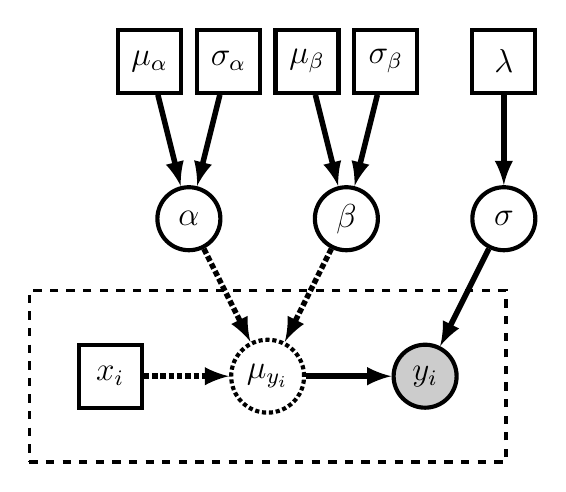
\begin{tikzpicture}
\node[obnode] (y) at (4,0) {\large $y_i$};
\node[snode] (sigma) at (5,2) {\large $\sigma$};
\node[constnode] (lambda) at (5,4) {\large $\lambda$};
\node[detnode] (muy) at (2,0) {\large $\mu_{y_i}$};
\node[snode] (beta) at (3,2) {\large $\beta$};
\draw[dtaro] (beta) -- (muy) ;
    \node[constnode] (mubeta) at (2.5,4) {\large $\mu_{\beta}$};
    \draw[taro] (mubeta) -- (beta) ;
    \node[constnode] (sigmabeta) at (3.5,4) {\large $\sigma_{\beta}$};
    \draw[taro] (sigmabeta) -- (beta) ;
\node[snode] (alpha) at (1,2) {\large $\alpha$};
\draw[dtaro] (alpha) -- (muy) ;
    \node[constnode] (mualpha) at (0.5,4) {\large $\mu_{\alpha}$};
    \draw[taro] (mualpha) -- (alpha) ;
    \node[constnode] (sigmaalpha) at (1.5,4) {\large $\sigma_{\alpha}$};
    \draw[taro] (sigmaalpha) -- (alpha) ;
\node[constnode] (x) at (0,0) {\large $x_i$};
\draw[taro] (muy) -- (y) ;
\draw[dtaro] (x) -- (muy) ;
\draw[taro] (sigma) -- (y) ;
\draw[taro] (lambda) -- (sigma) ;
\node[rectangle, dashed, very thick, inner sep=6mm, draw=black!100, fit=(y)(muy)(x)] (plate) {};
\end{tikzpicture}
\end{document}
